%\section{Approach}

\section{Architecture}

\subsection{Overview}

Our work adds to the current cellular network two main components: a SDN substrate,   
and a registration and control server (cloud manager in figure ~\ref{fig:architecture}). 
The SDN substrate locates in between the Radio Access Network (RAN) 
and the cellular core network that intercepts and reroutes offloading traffic to the offloading 
server(s) inside the core. This substrate consists of Openflow switches (OFSes) 
that talk to eNodeBs via GTP tunnels and to offloading servers via regular 
IP connections. The substrate is controlled by controller(s) to
realize traffic rerouting. The cloud manager maintains a database of registered offloading services 
and is responsible for allocating offloading servers inside the core. It also exposes 
to users an interface to register for offloading services and performs other functions such as 
charging and security.

\begin{figure}[hbtp]
\centering
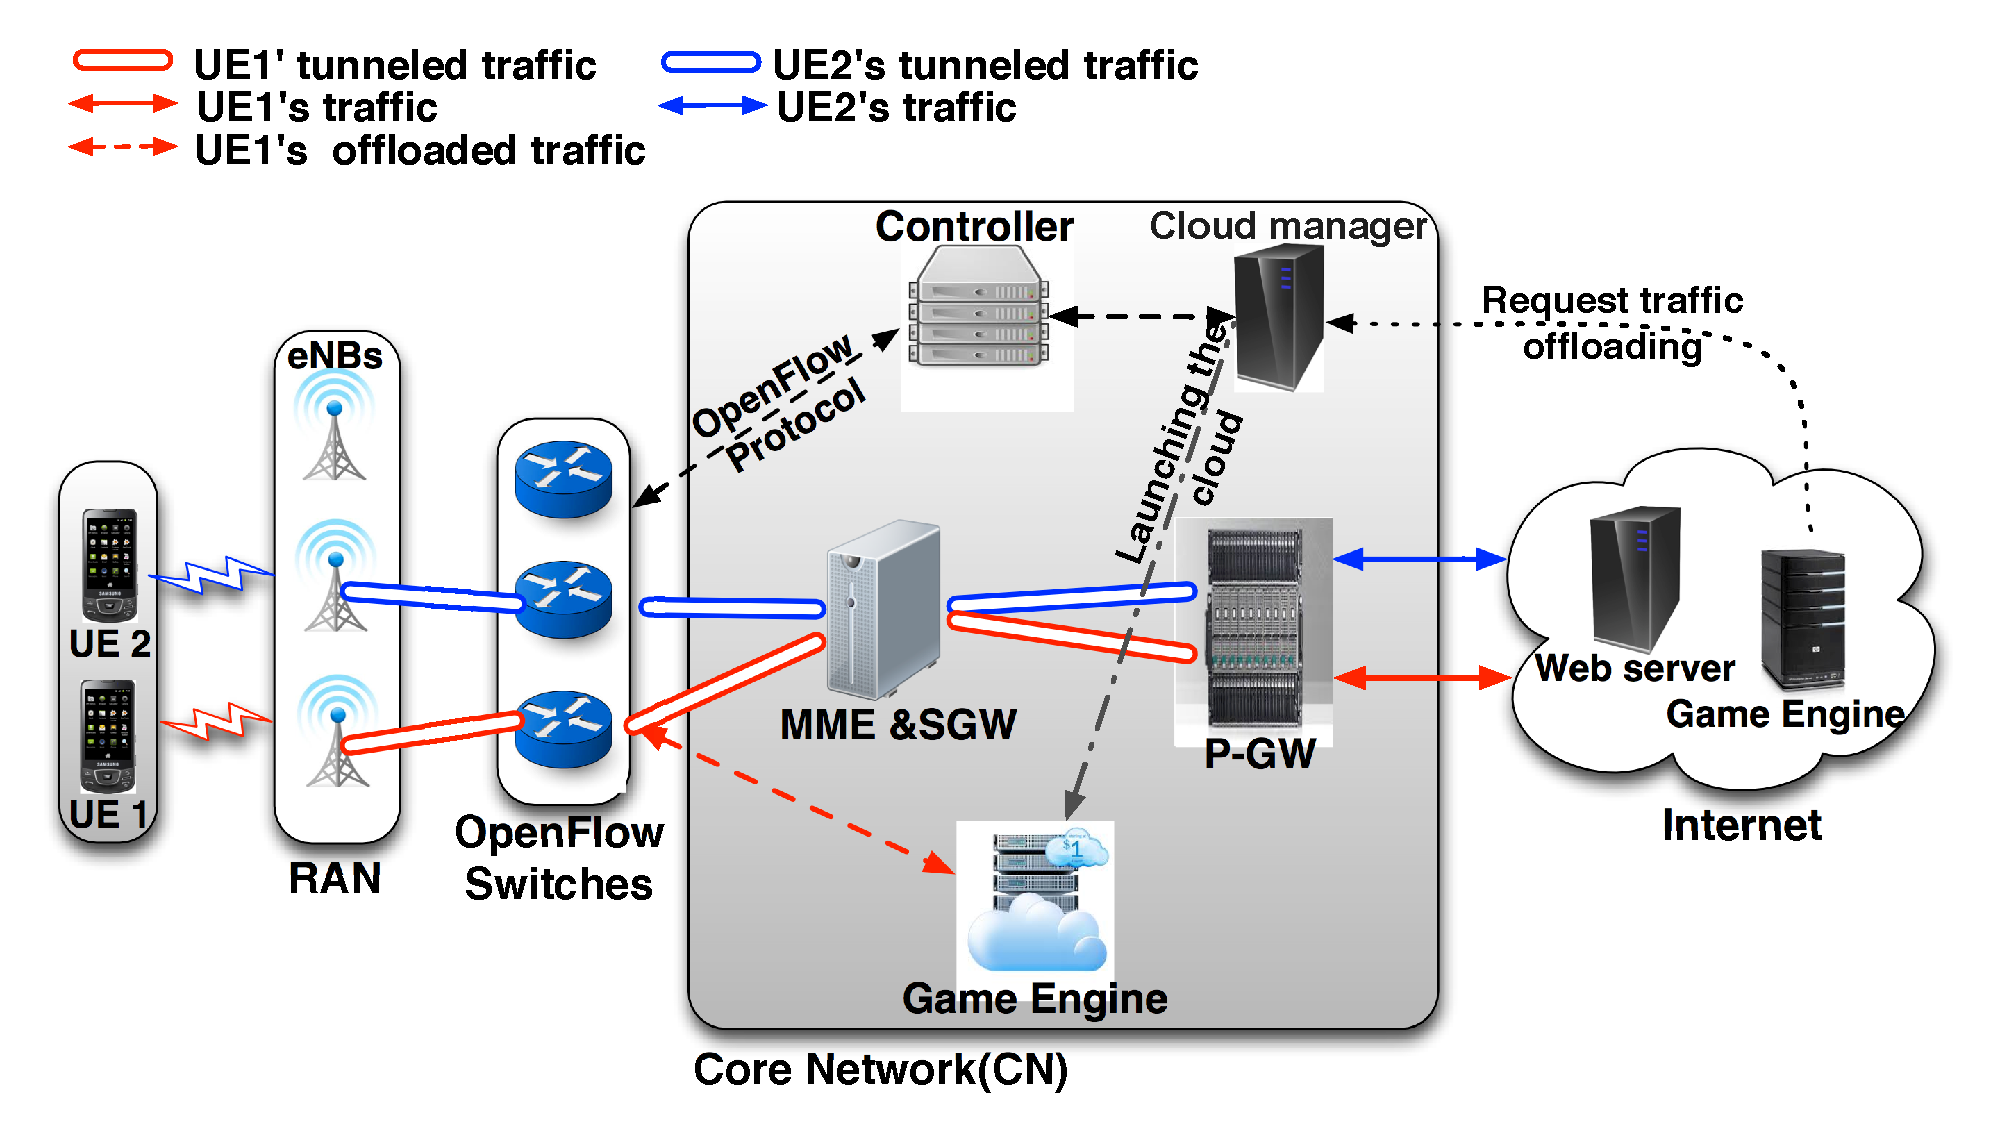
\includegraphics[scale=0.24]{./figure/architecture_mobi}
\caption{System architecture}
\label{fig:architecture}
\end{figure}

A basic work-flow of the system is described as follow: users (e.g, game providers) 
contact the cloud manager to register offloading functionality for their services. The cloud manager 
allocates offloading server(s) and notifies the SDN controller(s) about the offloading server(s) and the registered 
traffic. The SDN controller then translates these information into SDN rules 
(e.i., match:actions) and installs these rules to the SDN substrate. Once these rules are deployed, the SDN substrate 
is able to reroute registered offloading traffic from/to RAN to/from appropriate offloading servers 
while leaving other unregistered traffic untouched.


\subsection{Realization}

\subsubsection{Cloud manager}

Cloud manager maintains information about offloading traffic and provides an 
interface that allows users to register for offloading functionality. Users can specify 
a traffic that will enjoy offloading beforehand or during operation (similar to 
traffic balancing concept when a server becomes overwhelmed or when the network condition is not 
favorable causing an increasing of delay and therefore offloading is needed). 
Ideally, users can further specify a certain QoS associated with a traffic. 
For example, a game provider registers IP(s) of game engine(s) that 
it wants to do offloading due to the delay requirement of the game or a bad network condition. 
This game provider can also specify guaranteed 
bit rate and delay budget for the engine(s). The game provider interacts with the cloud manager 
via an interface (e.g, web front-end) to register/modify these services.

\subsubsection{SDN substrate}

SDN substrate is a set of Openflow switches (OFSes) controlled by controller(s) that 
realizes the offloading (as in figure ~\ref{fig:architecture})
Traffic from RAN are intercepted by this substrate and applied offloading rules if 
needed. An OFS acts like an access switch (AS) that 
maintains GTP tunnels with eNodeBs and performs GTP encapsulation/de-capsulation 
and contacts its controller to query for offloading rules. The AS also 
performs packet classification to map and translate IP packets to GTP tunneling.\\

After going through an AS, packets are pure IPs and therefore could be routed 
using regular IP routing. Current Openflow switches do not support 
packet payload matching and therefore can not forward 
packets based on GTP tunneling information. Therefore, the pipeline of an OFS should be 
modified to be able to de-capsulate incoming GTP packets before handing them to 
the regular OFS's pipeline (IP packet matching and action).\\

\subsubsection{Packet offloading}

When attaches to the network for the first time, 
an UE follows a normal attaching process (e.g,
authentication, bearers establishment, and IP address acquiring 
from the PGW). After resources are 
allocated, the UE can talk to an Internet server using the 
server's IP address. Traffic from UE, however, are 
not entirely routed to the Internet as usual but intercepted 
by the AS and offloading traffic 
are rerouted to the appropriate local offloading server.
(dotted arrow in Figure ~\ref{fig:architecture}).\\

An example of packet processing in an uplink direction could be described 
as follow: packets from an UE are sent by eNodeB to the 
AS in a GTP encapsulated form. These are UDP packets that have eNodeB's IP as 
the source IP address and SGW's IP as the destination IP address. At the beginning of a connection, 
AS forwards the first GTP packet to its controller for processing. The controller strips the outer GTP header of 
the original UDP packet to reveal the inner IP packet 
(the source and destination IP addresses of the inner IP packet 
are UE's IP and the remote server's IP respectively). It then compares 
the destination IP of this packet with its offloading database. A match 
means offloading service is applicable for this flow and 
therefore a flow entry will be installed into the AS to process future incoming packets. 
The flow entry in the AS replaces the source IP address of the incoming packets with the 
AS's IP and the destination IP address with the offloading server's IP. 
At the offloading server's perspective, it is communicating with the AS but not the eNodeB. 
Since the AS acts similarly to an network address translator (NAT), the controller has 
to store GTP's header information such as GTP message type and TEID (tunnel ID) 
for encapsulating returning packets in the downlink direction.\\

For downlink traffic, the AS encapsulates returning IP packets to 
create UDP packets with appropriate GTP headers to send to eNodeBs. 
Similarly, a flow entry is installed into the AS to reform 
the returning IP packets to UDP/GTP packets that match the original uplink tunnel (as described in the last 
paragraph). These actions include changing the source IP and destination IP addresses of the returning IP 
packets to SGW's IP 
and eNodeB's IP and placing correct GTP TEID (as what received in uplink direction). 
The mapping between returning packets and  
GTP TEID could be done using port number (AS could be seen as a NAT).






